\section{Aufgabe 18}
\setcounter{section}{18}

\begin{enumerate}[1.]
    \item Es seien $A := [0,1] \cup [2,3]$ und $B := [\dfrac{1}{2},
        \dfrac{3}{2}]$.

        \begin{enumerate}[(a)]
            \item Skizzieren Sie den Graph von $f : [0,5] \longrightarrow
                \mathbb{R}$ mit $f(x) := \mathds{1}_A(x) + \mathds{1}_B(x)$

                Siehe Abbildung~\ref{fig:abbildung-18-01}

                \begin{figure}[p]
                    \centering
                    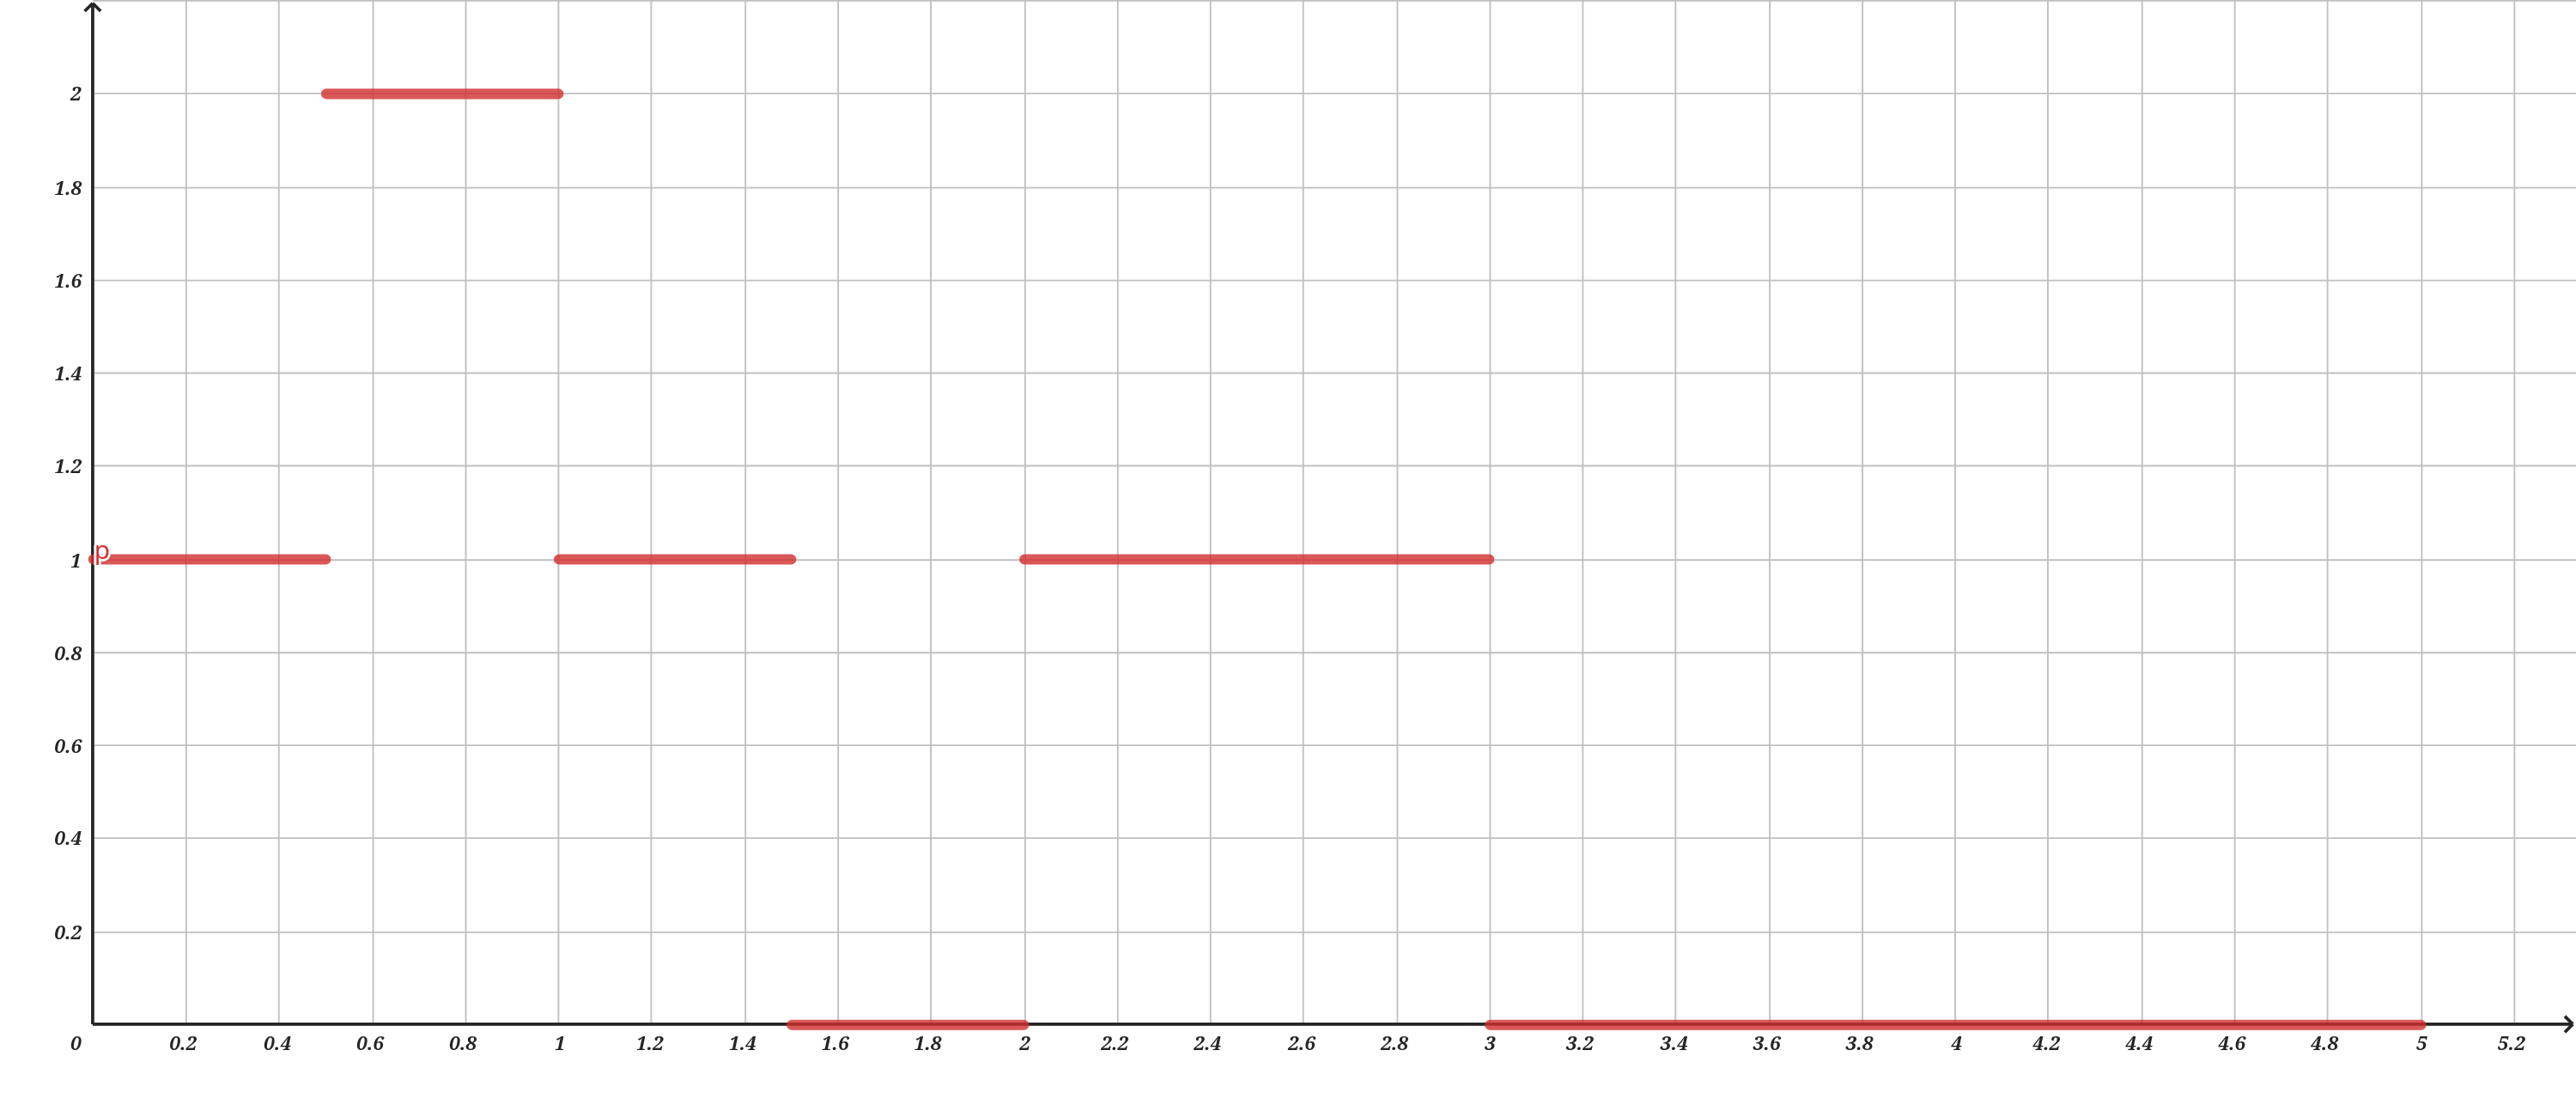
\includegraphics[width=0.9\textwidth]{./assets/abbildung-18-01.png}
                    \caption{$f(x) := \mathds{1}_A(x) + \mathds{1}_B(x)$}
                    \label{fig:abbildung-18-01}
                \end{figure}

            \item Skizzieren Sie den Graph von $g: [0, 5] \longrightarrow
                \mathbb{R}$ mit $g(x) := \mathds{1}_A(x) - \mathds{1}_B(x)$

                Siehe Abbildung~\ref{fig:abbildung-18-02}

                \begin{figure}[p]
                    \centering
                    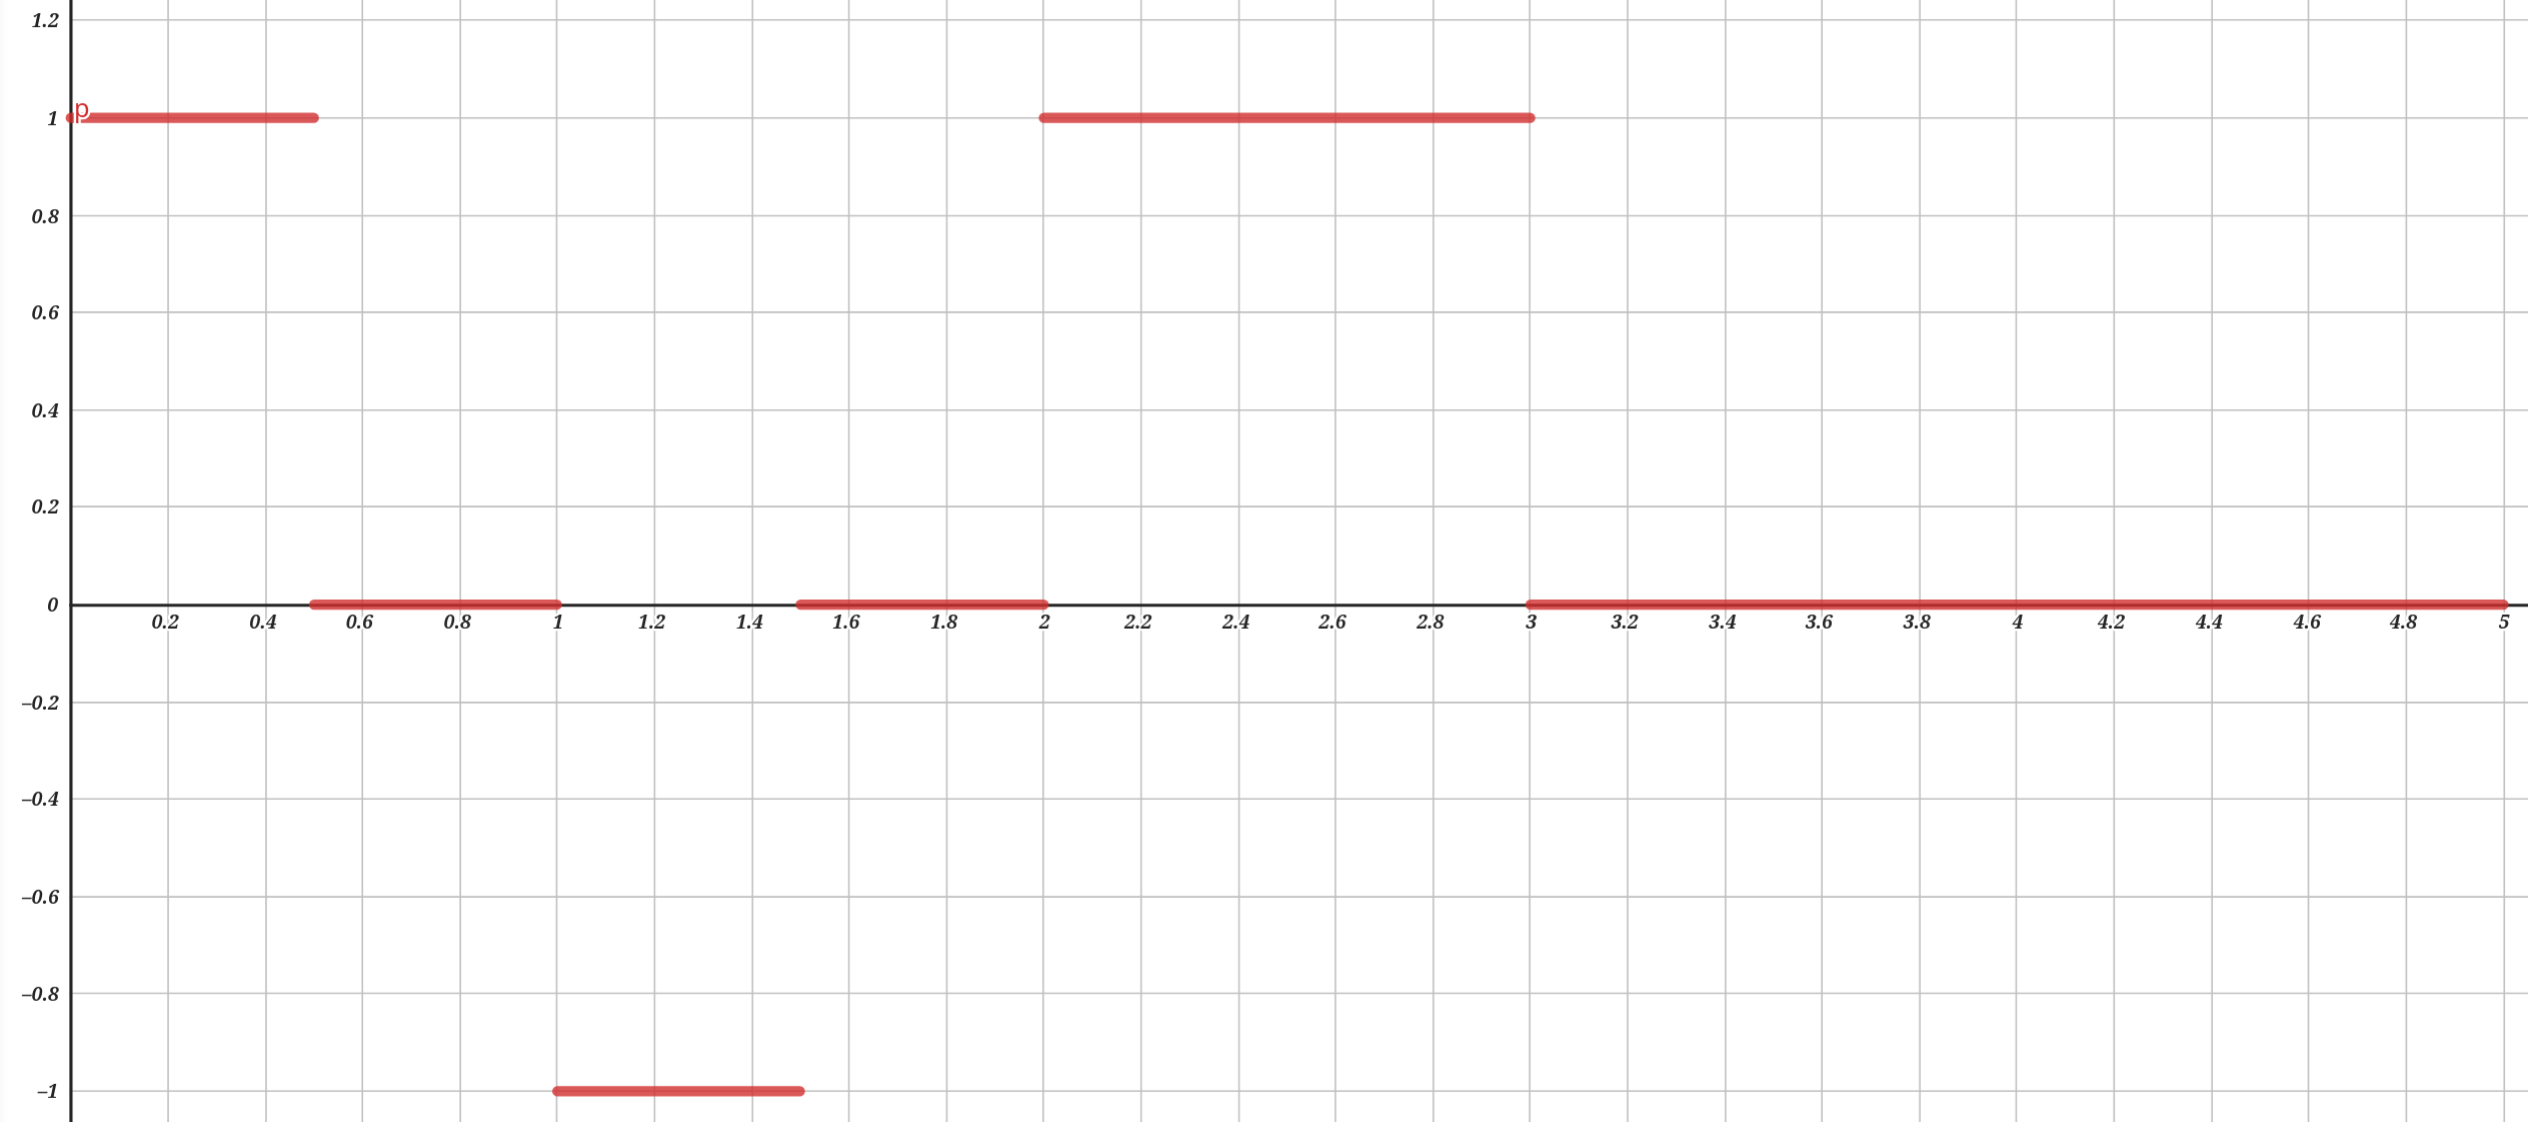
\includegraphics[width=0.9\textwidth]{./assets/abbildung-18-02.png}
                    \caption{$g(x) := \mathds{1}_A(x) - \mathds{1}_B(x)$}
                    \label{fig:abbildung-18-02}
                \end{figure}
        \end{enumerate}
\end{enumerate}
